
\chapter{Iteración }

\index{iteración}

\section{Asignación múltiple}

\index{asignación} \index{sentencia!asignación} \index{asignación múltiple}

Puede que usted ya haya descubierto que es posible realizar más de
una asignación a la misma variable. Una nueva asignación hace que
la variable existente se refiera a un nuevo valor (y deje de referirse
al viejo valor).

\inputencoding{latin9}\begin{lstlisting}
pedro = 5
print(pedro)
pedro = 7
print(pedro)
\end{lstlisting}
\inputencoding{utf8} La salida de este programa es:

\texttt{5 }

\texttt{7} 

porque la primera vez que \texttt{pedro} se imprime, tiene el valor
5, y la segunda vez tiene el valor 7.

Aquí se puede ver cómo luce la \textbf{asignación múltiple } en un
diagrama de estado:

\beforefig \centerline{
\includegraphics{illustrations/assign2}}
\afterfig

Con asignación múltiple es muy importante distinguir entre una asignación
y una igualdad. Como Python usa el signo igual (\texttt{=}) para la
asignación podemos caer en la tentación de interpretar a una sentencia
como \texttt{a = b} como si fuera una igualdad. ¡Y no lo es!

Primero, la igualdad es conmutativa y la asignación no lo es. Por
ejemplo, en la matemática si $a=7$ entonces $7=a$. Pero en Python,
la sentencia \texttt{a = 7} es legal aunque \texttt{7 = a} no lo es.

Además, en matemática, una sentencia de igualdad \textit{siempre}
es cierta. Si $a=b$ ahora, entonces $a$ siempre será igual a $b$.
En Python, una sentencia de asignación puede lograr que dos variables
sean iguales pero sólo por un tiempo determinado:

\inputencoding{latin9}\begin{lstlisting}
a = 5
b = a    # a y b ahora son iguales
a = 3    # a y b no son iguales ahora
\end{lstlisting}
\inputencoding{utf8} La tercera línea cambia el valor de \texttt{a} pero no cambia el
valor de \texttt{b}, así que ya no serán iguales. En algunos lenguajes
de programación se usa un signo diferente para la asignación como
\texttt{<-} o \texttt{:=} para evitar la confusión.

Aunque la asignación múltiple puede ser útil se debe usar con precaución.
Si los valores de las variables cambian frecuentemente se puede dificultar
la lectura y la depuración del código.

\section{La sentencia \texttt{while (mientras)} }

\index{sentencia while} \index{sentencia!while} \index{ciclo!while}
\index{iteración}

Los computadores se usan a menudo para automatizar tareas repetitivas.
Esto es algo que los computadores hacen bien y los seres humanos hacemos
mal.

Hemos visto dos programas, \texttt{nLineas} y \texttt{conteo}, que
usan la recursión para lograr repetir, lo que también se denomina
\textbf{iteración}. Como la iteración es tan común, Python proporciona
varios elementos para facilitarla. El primero que veremos es la sentencia
\texttt{while}.

Aquí presentamos a la función \texttt{conteo} usando una sentencia
\texttt{while}:

\inputencoding{latin9}\begin{lstlisting}
def conteo(n):
  while n > 0:
    print(n)
    n = n-1
  print("Despegue!")
\end{lstlisting}
\inputencoding{utf8} Como eliminamos el llamado recursivo, esta función deja de ser recursiva.

La sentencia \texttt{while} se puede leer como en el lenguaje natural.
Quiere decir, ``Mientras \texttt{n} sea mayor que 0, continúe desplegando
el valor de \texttt{n} y reduciendo el valor de \texttt{n} en 1. Cuando
llegue a 0, despliegue la cadena \texttt{Despegue!}''.

Más formalmente, el flujo de ejecución de una sentencia \texttt{while}
luce así:
\begin{enumerate}
\item Evalúa la condición, resultando en \texttt{False} (falso) o \texttt{True}
(cierto).
\item Si la condición es falsa (False), se sale de la sentencia \texttt{while}
y continúa la ejecución con la siguiente sentencia (afuera del while).
\item Si la condición es cierta (True), ejecute cada una de las sentencias
en el cuerpo y regrese al paso 1.
\end{enumerate}
El cuerpo comprende todas las sentencias bajo la cabecera que tienen
la misma indentación.

Este flujo se denomina \textbf{ciclo} porque el tercer paso da la
vuelta hacia el primero. Note que si la condición es falsa la primera
vez que se entra al while, las sentencias internas nunca se ejecutan.

\index{condición} \index{ciclo} \index{ciclo!cuerpo} \index{cuerpo!ciclo}
\index{ciclo infinito} \index{ciclo!infinito}

El cuerpo del ciclo debería cambiar el valor de una o más variables,
de forma que la condición se haga falsa en algún momento y el ciclo
termine. De otra forma, el ciclo se repetirá para siempre, obteniendo
un \textbf{ciclo infinito}. Una broma común entre los científicos
de la computación es interpretar las instrucciones de los champús,
``Aplique champú, aplique rinse, repita,'' como un ciclo infinito.

En el caso de \texttt{conteo}, podemos probar que el ciclo termina
porque sabemos que el valor de \texttt{n} es finito, y podemos ver
que va haciéndose más pequeño cada vez que el while itera (da la vuelta),
así que eventualmente llegaremos a 0. En otros casos esto no es tan
fácil de asegurar:

\inputencoding{latin9}\begin{lstlisting}
def secuencia(n):
  while n != 1:
    print(n),
    if n%2 == 0:        # n es par
      n = n/2
    else:               # n es impar
      n = n*3+1
\end{lstlisting}
\inputencoding{utf8} La condición para este ciclo es \texttt{n != 1}, así que se repetirá
hasta que \texttt{n} sea \texttt{1}, lo que hará que la condición
sea falsa.

En cada iteración del ciclo while el programa despliega el valor de
\texttt{n} y luego chequea si es par o impar. Si es par, el valor
de \texttt{n} se divide por 2. Si es impar el valor se reemplaza por
\texttt{n{*}3+1}. Si el valor inicial (del argumento) es 3, la secuencia
que resulta es 3, 10, 5, 16, 8, 4, 2, 1.

Como \texttt{n} aumenta algunas veces y otras disminuye, no hay una
demostración obvia de que \texttt{n} llegará a ser 1, o de que el
programa termina. Para algunos valores particulares de \texttt{n}
podemos demostrar la terminación. Por ejemplo, si el valor inicial
es una potencia de dos, entonces el valor de \texttt{n} será par en
cada iteración del ciclo hasta llegar a 1. El ejemplo anterior termina
con una secuencia así que empieza con 16.

Dejando los valores particulares de lado, la interesante pregunta
que nos planteamos es si podemos demostrar que este programa termina
para {\em todos} los valores de \texttt{n}. Hasta ahora, ¡nadie
ha sido capaz de probarlo {\em o} refutarlo!.

\section{Tablas}

\label{tables} \index{tabla} \index{logaritmo}

Una gama de aplicaciones donde los ciclos se destacan es la de generación
de información tabular. Antes de que los computadores existieran la
gente tenía que calcular logaritmos, senos, cosenos y otras funciones
matemáticas a mano. Para facilitar la tarea, los libros matemáticos
incluían largas tablas con los valores de dichas funciones. La creación
de las tablas era un proceso lento y aburridor, y tendían a quedar
con muchos errores.

Cuando los computadores entraron en escena, una de las reacciones
iniciales fue ``Esto es maravilloso! Podemos usar los computadores
para generar las tablas, de forma que no habrían errores''. Eso resultó
(casi) cierto, pero poco prospectivo. Poco después los computadores
y las calculadoras se hicieron tan ubicuos que las tablas se hicieron
obsoletas.

Bueno, casi. Para algunas operaciones los computadores usan tablas
de valores para obtener una respuesta aproximada y luego hacer mas
cálculos para mejorar la aproximación. En algunos casos, se han encontrado
errores en las tablas subyacentes, el más famoso ha sido el de la
tabla para realizar la división en punto flotante en los procesadores
Pentium de la compañía Intel.

\index{Intel} \index{Pentium}

Aunque una tabla logarítmica no es tan útil como en el pasado, todavía
sirve como un buen ejemplo de iteración. El siguiente programa despliega
una secuencia de valores en la columna izquierda y sus logaritmos
en la columna derecha: \inputencoding{latin9}
\begin{lstlisting}
import math
x = 1.0
while x < 10.0:
  print(x, '\t', math.log(x))
  x = x + 1.0
\end{lstlisting}
\inputencoding{utf8}
La cadena \verb+'\t'+ representa un carácter \textbf{tab} (tabulador).

A medida que los caracteres y las cadenas se despliegan en la pantalla
un marcador invisible denominado \textbf{cursor} lleva pista de dónde
va a ir el siguiente carácter. Después de una sentencia \texttt{print},
el cursor va al comienzo de la siguiente línea.

El carácter tabulador mueve el cursor hacia la derecha hasta que alcanza
un punto de parada (cada cierto número de espacios, que pueden variar
de sistema a sistema). Los tabuladores son útiles para alinear columnas
de texto, como la salida del anterior programa:
\begin{verbatim}
1.0     0.0
2.0     0.69314718056
3.0     1.09861228867
4.0     1.38629436112
5.0     1.60943791243
6.0     1.79175946923
7.0     1.94591014906
8.0     2.07944154168
9.0     2.19722457734
\end{verbatim}
Si estos valores parecen extraños, recuerde que la función \texttt{log}
usa la base \texttt{e}. Ya que las potencias de dos son importantes
en la ciencias de la computación, a menudo deseamos calcular logaritmos
en base 2. Para este fin podemos usar la siguiente fórmula:

\begin{equation}
\log_{2}x=\frac{log_{e}x}{log_{e}2}
\end{equation}

Cambiando la salida del ciclo a:\inputencoding{latin9}
\begin{lstlisting}
print(x, '\t',  math.log(x)/math.log(2.0))
\end{lstlisting}
\inputencoding{utf8}\begin{verbatim}
   resulta en:
1.0     0.0
2.0     1.0
3.0     1.58496250072
4.0     2.0
5.0     2.32192809489
6.0     2.58496250072
7.0     2.80735492206
8.0     3.0
9.0     3.16992500144
\end{verbatim}
Podemos ver que 1, 2, 4, y 8 son potencias de dos porque sus logaritmos
en base 2 son números enteros. Si deseamos calcular el logaritmo de
más potencias de dos podemos modificar el programa así:\inputencoding{latin9}
\begin{lstlisting}
x = 1.0
while x < 100.0:
  print(x, '\t', math.log(x)/math.log(2.0))
  x = x * 2.0
\end{lstlisting}
\inputencoding{utf8}
Ahora, en lugar de agregar algo a \texttt{x} en cada iteración del
ciclo, produciendo una serie aritmética, multiplicamos a \texttt{x}
por algo constante, produciendo una serie geométrica. El resultado
es:

\index{serie aritmética} \index{serie geométrica}
\begin{verbatim}
1.0     0.0
2.0     1.0
4.0     2.0
8.0     3.0
16.0    4.0
32.0    5.0
64.0    6.0
\end{verbatim}
Gracias a los caracteres tabuladores entre las columnas, la posición
de la segunda columna no depende del número de dígitos en la primera.

Puede que las tablas de logaritmos no sirvan en nuestros días, ¡pero
para los científicos de la computación saber las potencias de dos
sí es muy importante!.

\index{secuencia de escape}

El carácter diagonal invertido (backslash) \verb+'\'+ indica el comienzo
de una \textbf{secuencia de escape}. Estas secuencias se utilizan
para representar caracteres invisibles como tabuladores y nuevas líneas.
La secuencia \verb+'\n'+ representa una nueva línea.

Una secuencia de escape puede empezar en cualquier posición de una
cadena; en el ejemplo anterior, la secuencia de escape tabuladora
es toda la cadena.

¿Cómo cree que se representa un diagonal invertido en una cadena?

\section{Tablas de dos dimensiones}

\index{tabla!bidimensional}

Una tabla de dos dimensiones es una en la que los valores se leen
en la intersección de una fila y una columna. Una tabla de multiplicación
es un ejemplo familiar. Digamos que usted desea imprimir una tabla
de multiplicación para los valores del 1 al 6.

Una buena forma de empezar es escribir un ciclo que imprima los múltiplos
de 2, en una sola línea:\inputencoding{latin9}
\begin{lstlisting}
i = 1
while i <= 6:
  print(2*i, '   ',end=' ')
  i = i + 1

print()
\end{lstlisting}
\inputencoding{utf8}
La primera línea inicializa una variable llamada \texttt{i}, que actúa
como un contador o \textbf{variable de ciclo}. A medida que se ejecuta
el ciclo, el valor de \texttt{i} se incrementa de 1 a 6. Cuando \texttt{i}
es 7, el ciclo termina. En cada iteración del ciclo despliega el valor
\texttt{2{*}i}, seguido de tres espacios.

El uso de \texttt{end=' '} en la función \texttt{print} cambia el
último caracter que se imprime, que por defecto es el de fin de línea.
Después de que el ciclo termina la segunda sentencia \texttt{print}
comienza una nueva línea.

La salida del programa es:
\begin{verbatim}
2      4      6      8      10     12
\end{verbatim}
Hasta aquí vamos bien. El paso siguiente es \textbf{encapsular} y
\textbf{generalizar}.

\section{Encapsulamiento y generalización}

\label{encapsulation}

\index{encapsulamiento} \index{generalización} \index{desarrollo de programas!encapsulamiento}
\index{desarrollo de programas!generalización}

Encapsular es el proceso de envolver un trozo de código en una función,
permitiendo tomar ventaja de todas los beneficios que esto conlleva.
Usted ha visto dos ejemplos de encapsulamiento: \texttt{imprimirParidad}
en la Sección~\ref{alternative execution}; y \texttt{esDivisible}
en la Sección~\ref{boolean}.

La generalización es tomar algo específico, tal como imprimir los
múltiplos de 2, y convertirlo en algo más general, tal como imprimir
los múltiplos de cualquier entero.

Esta función encapsula el ciclo anterior y lo generaliza para imprimir
múltiplos de un parámetro \texttt{n}:\inputencoding{latin9}
\begin{lstlisting}
def imprimaMultiplos(n):
  i = 1
  while i <= 6:
    print(n*i, end='\t')
    i = i + 1
  print()
\end{lstlisting}
\inputencoding{utf8}
Para encapsular el ciclo, todo lo que agregamos fue la primera línea
que declara el nombre de la función y la lista de parámetros. Para
generalizar, lo que hicimos fue reemplazar el valor 2 con el parámetro
\texttt{n}.

Si llamamos a esta función con el argumento 2, obtenemos la misma
salida de la sección anterior. Con el argumento 3, la salida es:
\begin{verbatim}
3      6      9      12     15     18
\end{verbatim}
Con el argumento 4, la salida es:
\begin{verbatim}
4      8      12     16     20     24
\end{verbatim}
Ahora, usted probablemente imagine cómo imprimir una tabla de multiplicación
—llamando a \texttt{imprimaMultiplos} repetidamente con diferentes
argumentos. De hecho, podemos usar otro ciclo:

\inputencoding{latin9}\begin{lstlisting}
i = 1
while i <= 6:
  imprimaMultiplos(i)
  i = i + 1
\end{lstlisting}
\inputencoding{utf8}
Observe lo similar que es este ciclo al ciclo interno de la función
\texttt{imprimaMultiplos}. Todo lo que hicimos fue reemplazar la sentencia
\texttt{print} con un llamado de función.

La salida de este programa es una tabla de multiplicación:
\begin{verbatim}
1      2      3      4      5      6
2      4      6      8      10     12
3      6      9      12     15     18
4      8      12     16     20     24
5      10     15     20     25     30
6      12     18     24     30     36
\end{verbatim}

\section{Más encapsulamiento}

Para demostrar el encapsulamiento otra vez, tomemos el código de la
sección \ref{encapsulation} y envolvámoslo en una función:\inputencoding{latin9}
\begin{lstlisting}
def imprimirTablaMultiplicacion():
  i = 1
  while i <= 6:
    imprimaMultiplos(i)
    i = i + 1
\end{lstlisting}
\inputencoding{utf8}
Este proceso es un \textbf{plan de desarrollo} común. Desarrollamos
código escribiendo líneas afuera de cualquier función o digitándolas
en el intérprete. Cuando funcionan, las ponemos dentro de una función.

Este plan de desarrollo es particularmente útil si usted no sabe,
cuando está empezando a programar, cómo dividir el programa en funciones.
Este enfoque permite diseñar a medida que se escribe código.

\section{Variables locales}

\index{variable!local} \index{variable local}

Puede estar preguntándose cómo usamos la misma variable, \texttt{i}
en las dos funciones \texttt{imprimaMultiplos} y \texttt{imprimaTabla}.
¿No ocurren problemas cuando una de ellas cambia el valor de la variable?

La respuesta es no, porque la \texttt{i} en \texttt{imprimaMultiplos}
y la \texttt{i} en \texttt{imprimaTabla} {\em no} son la misma
variable.

Las variables creadas dentro de una definición de función son locales;
no se puede acceder a ellas fuera de su función ``casa''. Esto quiere
decir que usted tiene la libertad de tener múltiples variables con
el mismo nombre en tanto no pertenezcan a la misma función.

El diagrama de pila para este programa muestra que las dos variables
llamadas \texttt{i} no son la misma. Se pueden referir a valores diferentes,
y cambiar una de ellas no altera la otra.

\beforefig \centerline{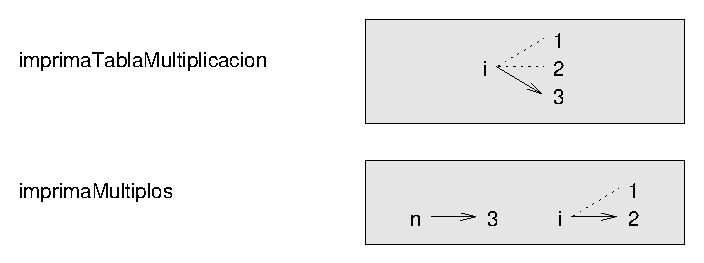
\includegraphics{illustrations/stack4}}
\afterfig

El valor de \texttt{i} en \texttt{imprimaTabla} va de 1 a 6. En el
diagrama va por el valor 3. En la próxima iteración del ciclo será
4. En cada iteración, \texttt{imprimaTabla} llama a \texttt{imprimaMultiplos}
con el valor actual de \texttt{i} como argumento. Ese valor se le
asigna al parámetro \texttt{n}.

Adentro de \texttt{imprimaMultiplos} el valor de \texttt{i} va de
1 a 6. En el diagrama, es 2. Cambiar esta variable no tiene efecto
en el valor de \texttt{i} en \texttt{imprimaTabla}.

Es legal y muy común tener diferentes variables locales con el mismo
nombre. Particularmente, nombres como \texttt{i} y \texttt{j} se usan
frecuentemente como variables de ciclo. Si usted evita usarlas en
una función porque ya las usó en otra, probablemente dificultará la
lectura del programa.

%\adjustpage{-2}%\pagebreak

\section{Mas generalización}

Como otro ejemplo de generalización, imagine que le piden un programa
que imprima una tabla de multiplicación de cualquier tamaño; no sólo
la tabla de seis por seis. Podría agregarse un parámetro a \texttt{imprimaTabla}:\inputencoding{latin9}
\begin{lstlisting}
def imprimaTabla(tope):
  i = 1
  while i <= tope:
    imprimaMultiplos(i)
    i = i + 1
\end{lstlisting}
\inputencoding{utf8}
Reemplazamos el valor 6 con el parámetro \texttt{tope}. Si llamamos
a \texttt{imprimaTabla} con el argumento 7, despliega:
\begin{verbatim}
1      2      3      4      5      6
2      4      6      8      10     12
3      6      9      12     15     18
4      8      12     16     20     24
5      10     15     20     25     30
6      12     18     24     30     36
7      14     21     28     35     42
\end{verbatim}
Esto está bien, pero quizás deseamos que la tabla sea cuadrada—con
el mismo número de filas y columnas. Para lograrlo, añadimos un parámetro
a imprimaMultiplos que especifique cuántas columnas debe tener la
tabla.

Sólo por confundir, vamos a nombrarlo \texttt{tope}, demostrando que
diferentes funciones pueden tener parámetros con el mismo nombre (igual
que las variables locales). Aquí está el programa completo:\inputencoding{latin9}
\begin{lstlisting}
def imprimaMultiplos(n, tope):
  i = 1
  while i <= tope:
    print(n*i, end='\t')
    i = i + 1
  print()

def imprimaTabla(tope):
  i = 1
  while i <= tope:
    imprimaMultiplos(i, tope)
    i = i + 1
\end{lstlisting}
\inputencoding{utf8}
Note que cuando agregamos el nuevo parámetro tuvimos que cambiar la
primera línea de la función (la cabecera), y también el lugar donde
la función se llama en \texttt{imprimaTabla}.

Como se esperaba, este programa genera una tabla cuadrada de siete-por-siete:
\begin{verbatim}
1      2      3      4      5      6      7
2      4      6      8      10     12     14
3      6      9      12     15     18     21
4      8      12     16     20     24     28
5      10     15     20     25     30     35
6      12     18     24     30     36     42
7      14     21     28     35     42     49
\end{verbatim}
Cuando se generaliza una función adecuadamente, a menudo se obtiene
un programa con capacidades que no se habían planeado. Por ejemplo,
podríamos aprovechar el hecho de que $ab=ba$, que causa que todas
las entradas de la tabla aparezcan dos veces para ahorrar tinta imprimiendo
solamente la mitad de la tabla. Para lograrlo sólo se necesita cambiar
una línea de \texttt{imprimaTabla}. Cambiamos:
\begin{verbatim}
    imprimaMultiplos(i, tope)
\end{verbatim}
por
\begin{verbatim}
    imprimaMultiplos(i, i)
\end{verbatim}
y se obtiene:
\begin{verbatim}
1
2      4
3      6      9
4      8      12     16
5      10     15     20     25
6      12     18     24     30     36
7      14     21     28     35     42     49
\end{verbatim}

\section{Funciones}

\index{función}

Ya hemos mencionado los ``beneficios de las funciones.'' Usted se
estará preguntado cuales son estos beneficios. Aquí hay algunos:
\begin{itemize}
\item Nombrar una secuencia de sentencias aumenta la legibilidad de los
programas y los hace más fáciles de depurar.
\item Dividir un programa grande en funciones permite separar partes de
éste, depurarlas aisladamente, y luego componerlas en un todo coherente.
\item Las funciones facilitan la recursión y la iteración.
\item Las funciones bien diseñadas resultan ser útiles para muchos programas.
Una vez que usted escribe y depura una, se puede reutilizar.
\end{itemize}

\section{Glosario}
\begin{description}
\item [{Asignación múltiple:}] realizar más de una asignación a una
misma variable durante la ejecución de un programa.
\item [{Iteración:}] la ejecución repetida de un grupo de sentencias, ya
sea en una función recursiva o en un ciclo.
\item [{Ciclo:}] una sentencia o grupo de sentencias que se ejecuta repetidamente
hasta que una condición de terminación se cumple.
\item [{Ciclo infinito:}] ciclo en el que la condición de terminación
nunca se cumple.
\item [{Cuerpo:}] las sentencias adentro de un ciclo.
\item [{Variable de ciclo:}] variable que se usa como parte de la condición
de terminación de un ciclo.
\item [{Tab:}] (tabulador) carácter especial que causa el movimiento del
cursor al siguiente punto de parada en la línea actual.
\item [{Nueva línea:}] carácter que causa que el cursor se mueva al principio
de la siguiente línea.
\item [{Cursor:}] marcador invisible que lleva pista de dónde se va a imprimir
el siguiente carácter.
\item [{Secuencia de escape:}] carácter de escape ($\backslash$) seguido
por uno o más caracteres imprimibles que se usan para denotar un carácter
no imprimible.
\item [{Encapsular:}] dividir un programa grande y complejo en componentes
(como funciones) y aislarlos entre sí (usando variables locales, por
ejemplo).
\item [{Generalizar:}] reemplazar algo innecesariamente específico (como
un valor constante) con algo general más apropiado (como una variable
o parámetro). La generalización aumenta la versatilidad del código,
lo hace más reutilizable y en algunos casos facilita su escritura.
\item [{Plan de desarrollo:}] proceso para desarrollar un programa. En
este capítulo demostramos un estilo de desarrollo basado en escribir
código que realiza cómputos simples y específicos, para luego encapsularlo
y generalizarlo.

\index{asignación múltiple} \index{asignación!múltiple} \index{iteración}
\index{ciclo!cuerpo} \index{ciclo} \index{ciclo infinito} \index{secuencia de escape}
\index{cursor} \index{tab} \index{nueva línea} \index{variable de ciclo}
\index{encapsular} \index{generalizar} \index{plan de desarrollo}
\index{programas!desarrollo de}
\end{description}

\section{Ejercicios}
\begin{enumerate}
\item Siga la ejecución de la última versión de \texttt{imprimaTabla} y
descifre cómo trabaja. 
\item Reescriba la función \texttt{nLineas} de la Sección \ref{recursion},
usando iteración en vez de recursión. 
\item Escriba una sola cadena que

\beforeverb 
\begin{verbatim}
produzca
        esta
                salida.
\end{verbatim}
\afterverb
\item Escriba un programa que despliegue las potencias de 2 hasta 65,536
(esto es $2^{16}$).
\item Escriba una función \verb+muestra_numeros_triangulares(n)+ que muestre
los primeros n números triangulares. Una llamada a \verb+muestra_numeros_triangulares(5)+
produciría la siguiente salida: \beforeverb 

\begin{verbatim}
  1       1
  2       3
  3       6
  4       10
  5       15
  
\end{verbatim}
\afterverb
\item Muchos cálculos de funciones matemáticas se realizan con series infinitas,
por ejemplo:

$\ln{x}=\sum_{n=1}^{\infty}\frac{1}{{n}}\left(\frac{x-1}{x}\right)^{n}=\left(\frac{x-1}{x}\right)+\frac{1}{2}\left(\frac{x-1}{x}\right)^{2}+\frac{1}{3}\left(\frac{x-1}{x}\right)^{3}+\cdots$

que son aproximadas fijando un valor $n$ tal que la precisión, dada
por el número de cifras significativas correctas del valor calculado,
sea buena. Escriba un programa que calcule el logaritmo natural de
un número dado basado en la formula anterior. Para esto debe probar
con varios valores de $n$ hasta que obtenga un buen número de cifras
significativas correctas comparando el resultado de su programa con
el de \verb+math.log+.
\item Busque una formula correcta para calcular el seno de un ángulo y escriba
un programa para calcular este valor basado en la formula, como en
el punto anterior. Compare con \verb+math.sin+.
\item Compare los valores de $n$ que obtuvo para los puntos 6 y 7. Explique
si encuentra diferencias.
\item Escriba una función, \verb+es_primo+, que tome un solo argumento
entero y devuelva \verb+True+ cuando el argumento es un número primo
y \verb+False+ en caso contrario.
\item Agregue el código para chequeo de tipo de datos y para las prueba
unitarias a todas las funciones desarrolladas previamente.
\end{enumerate}

